%% ---
%% Modelo de trabalhos com base nos modelos ABNTEX2, simplificado
%% Allex Lima - allexlima@unn.edu.br
%% ----


\documentclass[12pt, oneside, a4paper, english, brazil]{abntex2}

\usepackage{lmodern}
\usepackage[utf8]{inputenc}
\usepackage{indentfirst}
\usepackage{color}
\usepackage{graphicx}
\usepackage{subfig}
\usepackage{microtype}
\usepackage{amsmath}

\usepackage[brazilian,hyperpageref]{backref}
\usepackage[alf]{abntex2cite}
\graphicspath{ {files/images/} }

%% ---
%% Dados para CAPA e FOLHA DE ROSTO
%% ---

\titulo{Fonte de Conversão AC/DC}
\autor{
    Allex Lima - 14003147\\
    Daniel Bispo - 14257165\\
    Heryck Michael - 14126346\\
    Paulo Moraes - 12078549\\
    Renan Barroncas - 14043300
}
\orientador{Profº. M.Sc. Francisco Coelho}
\local{Manaus - AM}
\data{Novembro de 2016}

\instituicao{
    Centro Universitário do Norte - UniNorte Laureate\par
    Escola de Exatas \par
    Bacharelado em Engenharia da Computação
}

\preambulo{
    Relatório apresentado como complemento de entrega do 1º (primeiro) projeto da matéria Eletrônica Analógica e Digital, do Curso de Engenharia da Computação, no Centro Universitário do Norte - UniNorte Laureate.
    \par
    \vspace{\onelineskip}
    \imprimirorientador
}

\makeindex

\renewcommand{\imprimircapa}{%
    \begin{capa}%
        \center
        \ABNTEXchapterfont\large\textsc{\imprimirinstituicao}
        \vspace*{1.1cm}
        \par
        {\ABNTEXchapterfont\large\imprimirautor}
        \vfill
        \begin{center}
            {\ABNTEXchapterfont\Large\textsc{\imprimirtitulo}}
        \end{center}
        \vfill
        \large\imprimirlocal\
        \par
        \large\imprimirdata
        \vspace*{1cm}
    \end{capa}
}

\renewcommand{\imprimirfolhaderosto}{
    \begin{center}%
        {\ABNTEXchapterfont\large\imprimirautor}

        \vspace*{\fill}\vspace*{\fill}
        \begin{center}
            {\ABNTEXchapterfont\Large\textsc{\imprimirtitulo}}
        \end{center}
        \vspace*{\fill}

        \hspace{.45\textwidth}
        \begin{minipage}{.5\textwidth}
            \SingleSpacing
            \imprimirpreambulo
        \end{minipage}%
        \vspace*{\fill}

        \large\imprimirlocal
        \par
        \large\imprimirdata
        \vspace*{1cm}
    \end{center}
    \newpage
}

\renewcommand{\ABNTEXchapterfontsize}{\Large}
\renewcommand{\ABNTEXsubsectionfontsize}{\large}

% Configuração das referências
\renewcommand{\backrefpagesname}{}
\renewcommand{\backref}{}
\renewcommand*{\backrefalt}[4]{}

% Configuração das notas de rodapé
\renewcommand{\footnotesize}{\small}
\setlength{\skip\footins}{1.1cm}

\begin{document}

    \selectlanguage{brazil}    %Seleciona o idioma do documento
    \frenchspacing             %Retira espaço extra obsoleto entre as frases.

    %% ----------------------------------------------------------
    %% Elementos Pré-textuais
    %% ----------------------------------------------------------

    %% ---
    %% Capa e Folha de rosto
    %% ---

    \imprimircapa
    \imprimirfolhaderosto

    %% ---
    %% Abstract e Resumo
    %% ---
    %
    %\begin{resumo}[Abstract]
    %   \begin{otherlanguage*}{english}
    %    This is the english abstract.
    %
    %    \textbf{Keywords}: latex. abntex. text editoration.
    % \end{otherlanguage*}
    %\end{resumo}

    %\begin{resumo} %Resumo
    %    blablabla...
    %
    %    \textbf{Palavras-chave}: bla, bla e bla.
    %\end{resumo}

    %% ---
    %% Sumário
    %% ---

    \pdfbookmark[0]{\contentsname}{toc}
    \tableofcontents*
    \cleardoublepage

    % ----------------------------------------------------------
    % ELEMENTOS TEXTUAIS
    % ----------------------------------------------------------
    \textual

    %% ---
    %% Introdução (exemplo de capítulo sem numeração, mas presente no Sumário)
    %% ---

    \chapter*[Introdução]{Introdução}
    \addcontentsline{toc}{chapter}{Introdução}
        %% Descrição de, no máximo em 2 ou 3 parágrafos de 3..4 linhas, cada, no máximo, abordando:
%% - o que espera-se fazer, por quê?, onde será aplicado ~ (objetivos)
A construção de uma fonte AC/DC objetiva consolidar conhecimentos adquiridos na disciplina de Eletrônica Analógica e Digital que envolvem conversão de uma tensão alternada (AC), facilmente encontrada nas redes elétricas residenciais, para tensão contínua (DC), comumente encontrada em pilhas e baterias.
\par
Os conceitos dos elementos individuais do circuito, como os dos diodos retificadores e reguladores lineares, possuem uma teoria de alta relevância na matéria, sendo a construção da fonte o exercício prático mais indicado para o seu entendimento prático. A fonte AC/DC irá alimentar, em subprojetos posteriores, a placa de prototipagem conhecida como \textit{Arduíno} através de uma de suas 3 portas USB.

    \chapter{Materiais utilizados}
        %% Uma lista contendo todos os materiais inclusos no projeto
%% Descrição básica de cada componente e, se possível, o porquê da utilização deste
\begin{itemize}[noitemsep]
\item 1 Caixa de madeira
\item 1 Placa Universal 20x10cm
\item 2 Dissipadores de calor
\item 1 Fusível
\item 1 Porta Fusível
\item 1 Transformador TRAN-2P2S
\item 4 Diodos 1N4007
\item 1 Capacitor 1000 $\mu$F
\item 1 Capacitor 470 $\mu$F
\item 1 Regulador de Tensão 12V 7812
\item 1 Regulador de Tensão 9V 7809
\item 1 Regulador de Tensão 5V 7805
\item 1 Resistor 1K$\Omega$
\item 1 Resistor 470$\Omega$
\item 1 Resistor 330$\Omega$
\item 1 LED Azul
\item 1 LED Verde
\item 1 LED Amarelo
\item 4 Interruptores (Chaves)
\item 3 Saídas USB
\end{itemize}

    \chapter{Metodologia e resultados}
        %% - Foto do circuíto (Como resultado)
%% - Explicação de como a caixa foi feita (madeira), pintura (preta), adesivos ~ (Enfim, a metodologia)
%% - Explicação das saídas USBS (do porquê nós utilizamos ((porque são mais universais)), das cores dos leds de cada saída (Azul: 12V, Verde: 9V, Laranja: 5V)

\begin{figure}[h]
    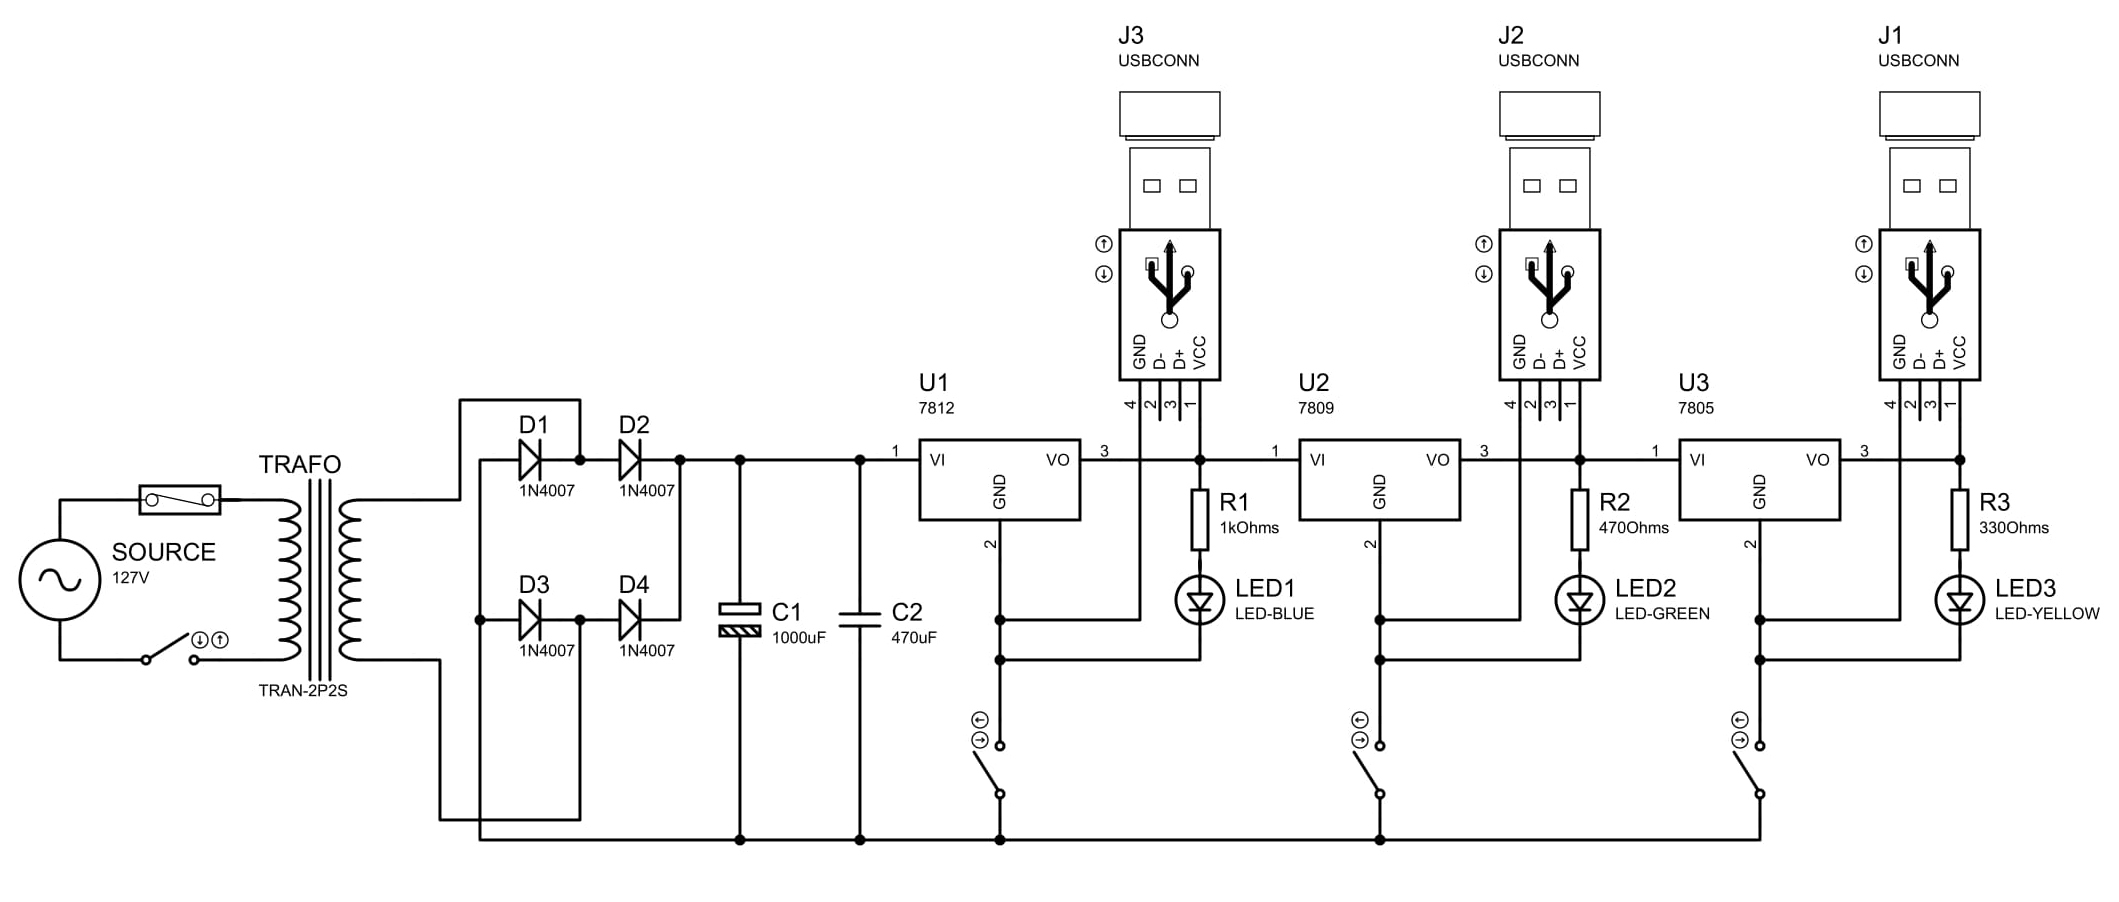
\includegraphics[height=7cm]{circuit-sketch}
    \caption{Desenho do Circuito Final}
    \label{fig:my_label}
\end{figure}

\par
A caixa na qual o circuito na placa universal foi comportada, é feita de madeira. Foram furados buracos correspondentes às saídas USB, os três LEDs (cada um acima de uma saída USB), furos para ventilar com ar externo e a entrada da energia AC. A caixa foi pintada com tinta da cor preta e adornada com adesivo contendo a logo e o nome do subprojeto.
\par
O motivo da utilização de saídas USB foi a universalidade, são mais comuns na atualidade para a função de fornecer energia à aparelhos eletrônicos como celulares, instrumentos musicais elétricos e \textit{modems}. Os LEDs de cores diferentes são úteis para diferenciar uma saída de outra. Todos esses aspectos proporcionam experiência simples para um usuário. O circuito representado na Figura 1 foi soldado na placa universal. \textit{Jumpers}, e até a própria solda em alguns casos, foram utilizados para estabelecer as conexões nos terminais positivos e negativos dos componentes.
\par
A primeira etapa do processo de conversão se situa na extremidade esquerda do circuito da Figura 1, a tensão que chegará através da tomada, podendo ser 110 volts ou 220 volts, será reduzida pelo transformador TRAN-2P2S para 18v, sendo ainda alternada. Em seguida, a regulagem da tensão é feita por diodos retificadores D1, D2, D3 e D4, transformando corrente alternada em contínua, apesar das oscilações. Depois disso é feita a filtragem capacitiva, utilizando os capacitores em paralelo, essa filtragem é capaz de estabilizar mais a corrente. Ainda sim exitem os chamados \textit{ripples}, que é uma pequena variação periódica residual da corrente contínua. Essa variação que ocorre a cada ciclo, é derivada dos tempos de carga e descarga dos capacitores. Já próximos às saídas, os reguladores de tensão linear mantém uma voltagem de saída constante.
    
    % ---
    % Conclusão
    % ---
    
    \chapter*[Conclusão]{Conclusão}
    \addcontentsline{toc}{chapter}{Conclusão}
        %% Breve relato do que foi observado durante o projeto e o que ainda pode ser melhorado
%% Onde será utilizada, etc 
O experimento de construção da fonte AC/DC foi crucial para o entendimento da conversão de corrente alternada para corrente contínua. A experiência permitiu observação em tempo real de como os componentes estudados nas aulas de Eletrônica Analógica e Digital interagem em conjunto para concretizar a conversão das correntes.
\par
O produto final dessa experiência irá viabilizar novos projetos da matéria, uma vez que irá alimentar um dispositivo \textit{Arduíno}. Isso irá demonstrar, mais uma vez, uma aplicação cotidiana do processo de conversão de corrente alternada para corrente contínua.


\end{document} 
